\subsection{Dispatcher and job scheduler}

\begin{frame}{Core component}

    The core of \express{} is its dispatching system,
    which is implemented by
    \href{https://github.com/MineralsCloud/SimpleWorkflows.jl}{\texttt{SimpleWorkflows.jl}},
    taking inspiration from
    \href{https://github.com/invenia/Dispatcher.jl}{\texttt{Dispatcher.jl}}
    (currently unmaintained) and
    \href{https://github.com/cihga39871/JobSchedulers.jl}{\texttt{JobSchedulers.jl}}.

    \begin{columns}[t]
        \begin{column}{0.4\textwidth}
            \begin{center}
                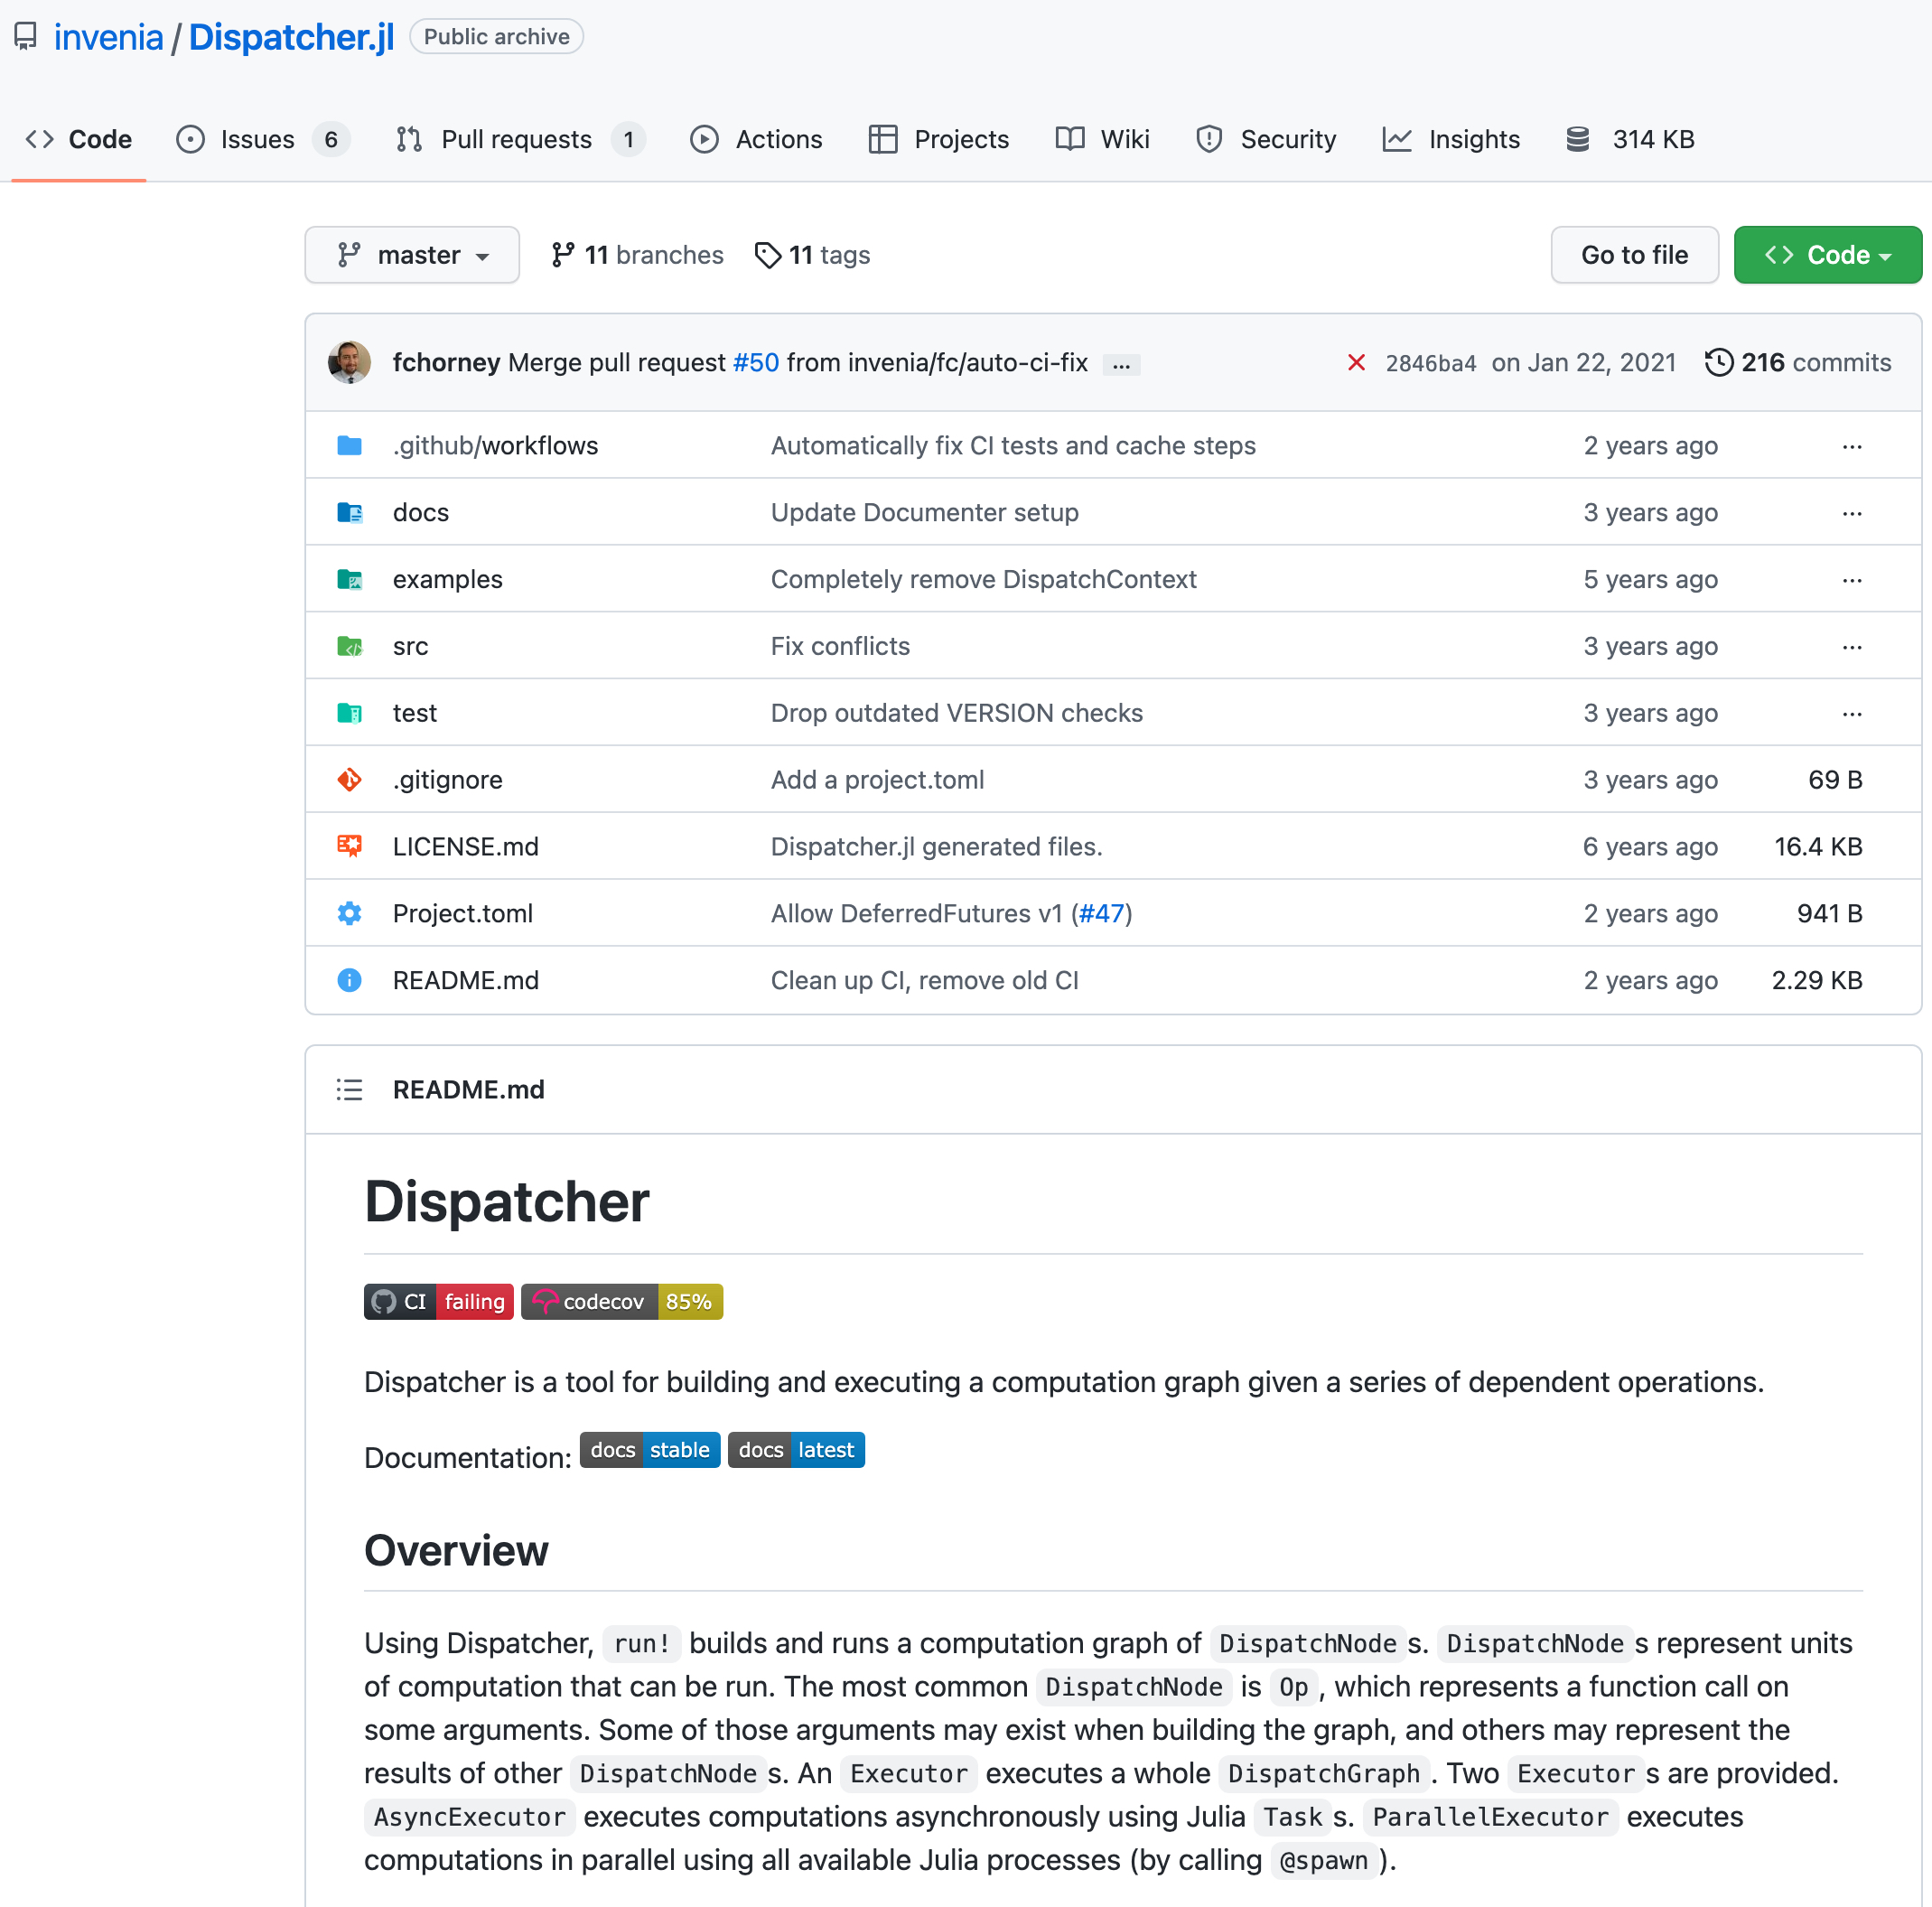
\includegraphics[height=0.5\textheight]{Dispatcher}
            \end{center}
        \end{column}
        \hfill
        \begin{column}{0.4\textwidth}
            \begin{center}
                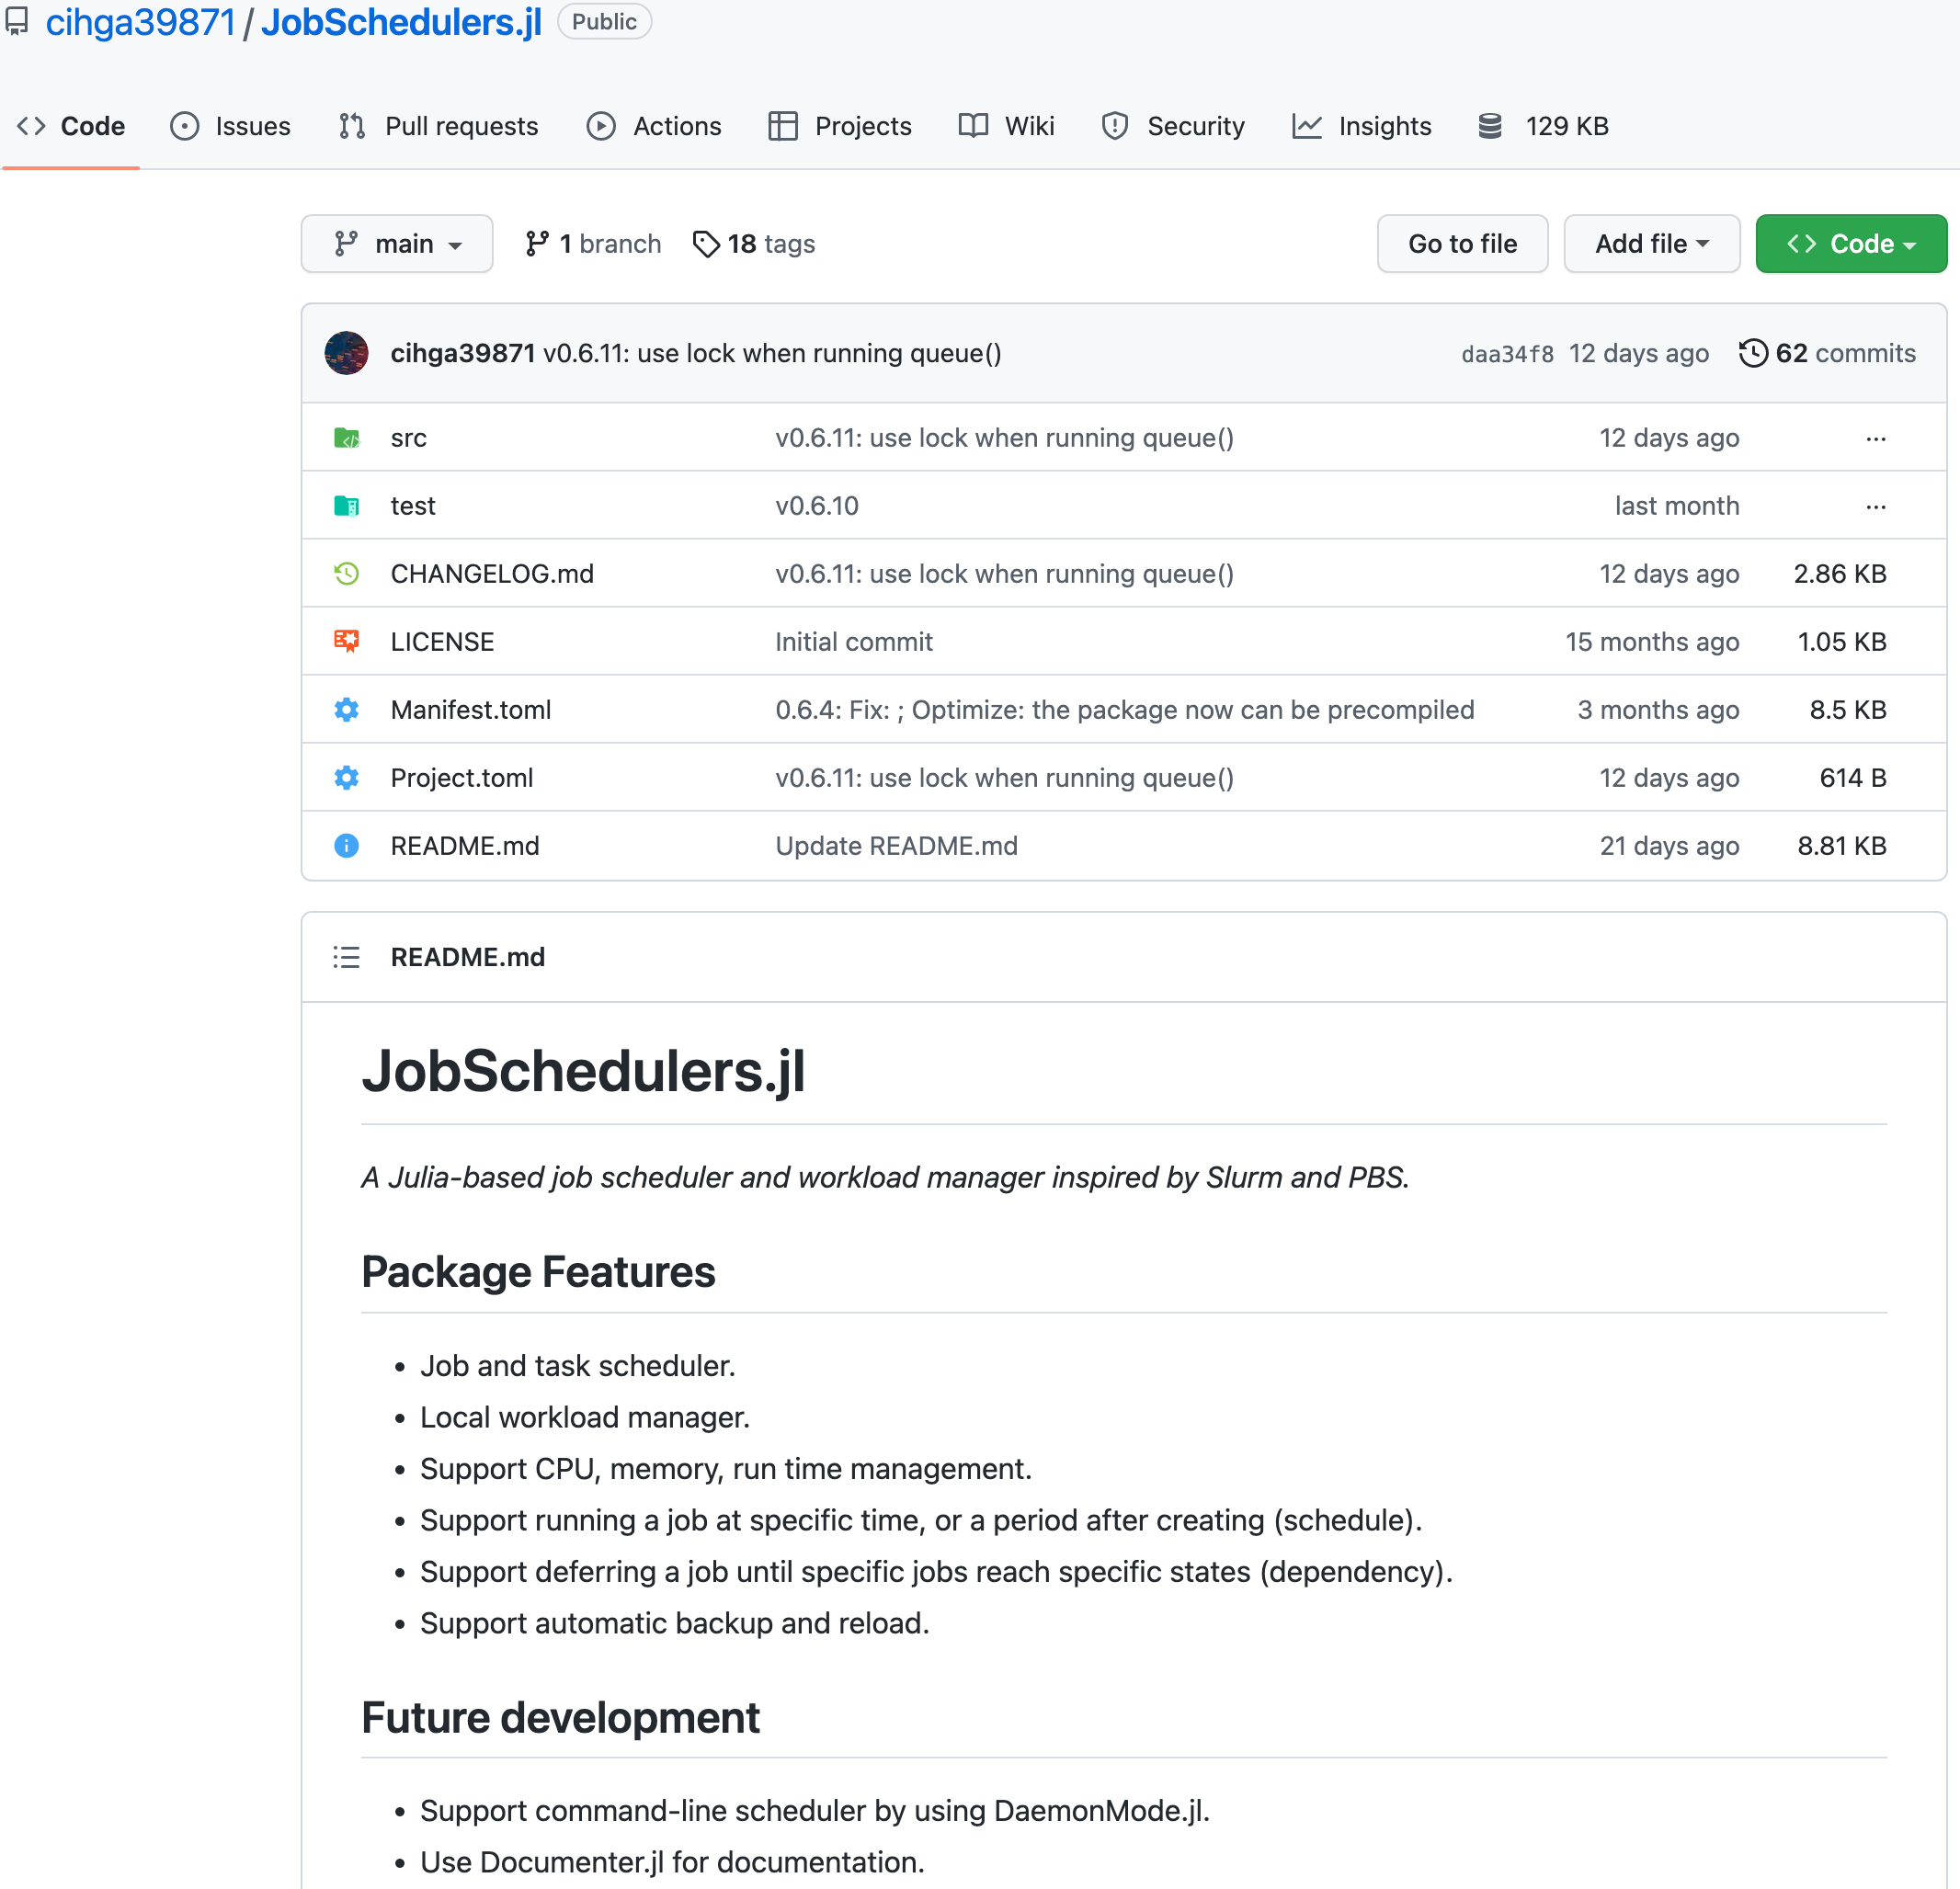
\includegraphics[height=0.5\textheight]{JobSchedulers}
            \end{center}
        \end{column}
    \end{columns}

\end{frame}

\begin{frame}{Design overview}

    The simplest atomic operation in a \texttt{Workflow} is called a \texttt{Job}.
    It tracks the time, result, and other info of the user's input.
    The relationship between each \texttt{Job} in the \texttt{Workflow} is represented by a
    DAG.
    To construct a \texttt{Workflow}, we provide some operators to simplify this step.

\end{frame}

% [fragile] needed when the content contains juliaverbatim.
\begin{frame}[fragile, allowframebreaks]{An example}

    Let's construct an arbitrary \texttt{Workflow}:
    {\scriptsize
    \begin{algorithmblock}
        \begin{juliaverbatim}
            using SimpleWorkflows
            i = @job (println("Start job `i`!"); sleep(5)) user = "me" desc = "i"
            j = @job (println("Start job `j`!"); sleep(3); exp(2)) user = "me" desc = "j"
            k = @job (println("Start job `k`!"); sleep(6)) desc = "k"
            l = @job (println("Start job `l`!"); run(`sleep 3`)) desc = "l" user = "me"
            m = @job (println("Start job `m`!"); sleep(3); sin(1)) desc = "m"
            n = @job (println("Start job `n`!"); run(`pwd` & `ls`)) user = "me" desc = "n"
            i → l
            j → k → m → n
            j → l
            k → n
            wf = Workflow(k)
        \end{juliaverbatim}
    \end{algorithmblock}
    }

    \framebreak

    The DAG of the \texttt{Job}s from \texttt{i} to \texttt{n} is

    \begin{figure}[H]
        \centering
        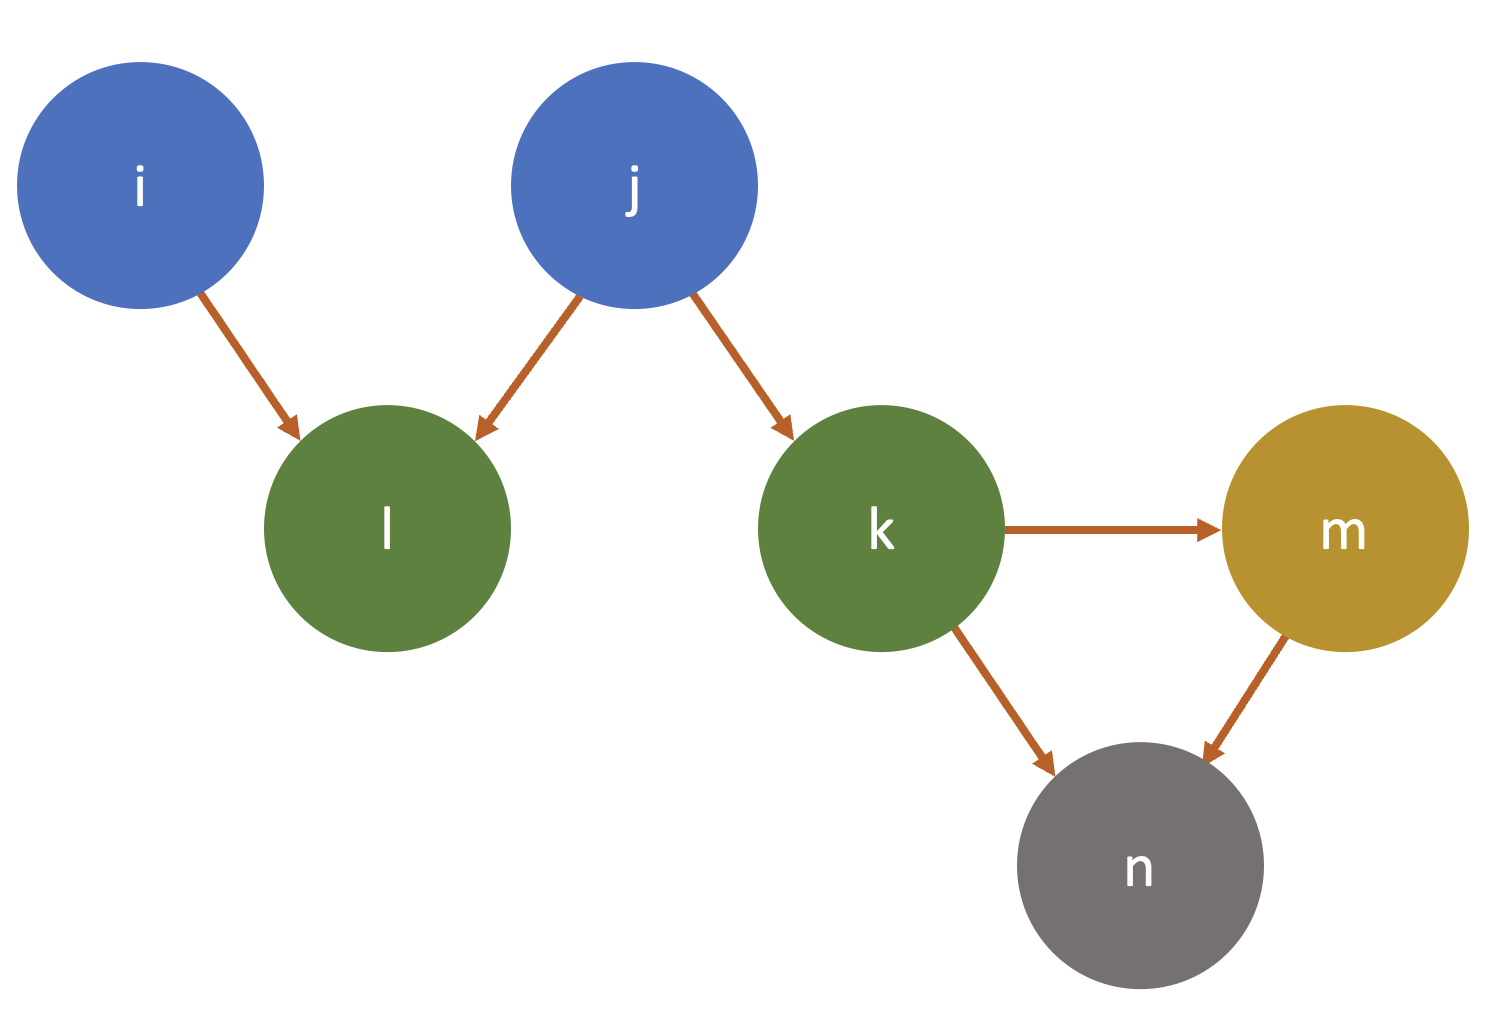
\includegraphics[height=0.45\textheight]{order}
        \caption{The execution order of the \texttt{Job}s from \texttt{i} to \texttt{n}.
            Blue circles are the first, then green, then yellow, and gray is the last.}
        \label{fig:order}
    \end{figure}

    \texttt{Jobs} of the same order are executed in parallel or asynchronously by
    Kahn's algorithm.

    \framebreak

    After or during the execution of the \texttt{Workflow}, we can use \texttt{queue} to
    print all the \texttt{Job}s' information:

    {\scriptsize
    \begin{algorithmblock}
        \begin{juliaverbatim}
            run!(wf)
        \end{juliaverbatim}
    \end{algorithmblock}
    }

    \begin{figure}[H]
        \centering
        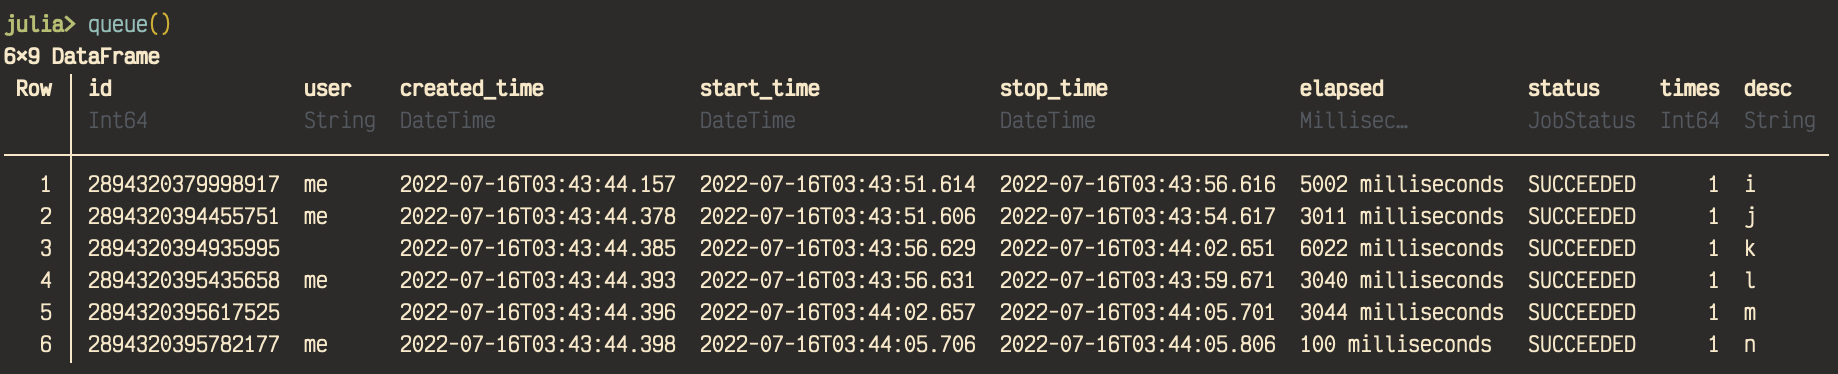
\includegraphics[width=0.8\textwidth]{queue}
        \caption{Queuing the information of the \texttt{Job}s in a \texttt{Workflow}.}
        \label{fig:queue}
    \end{figure}

    And a \texttt{JLD2} format file will be saved during this step. If some errors happened
    during the running or the execution is interrupted, we can rerun only the
    failed/interrupted \texttt{Jobs} according to the information saved in that file.

\end{frame}
